\chapter{Development}

\section{Experiment Design}
The following section explains how the different experiments were conducted in detail. When desinging the experiments, the focus on put on comparability rather than optimally tuned neural networks.  Further, it is shown how the datasets and anomalies were engineered.

\subsection{Title}
The following subsection give information on the chosen setups of the experiments that apply to all experiments, except where specifically stated otherwise.

\subsubsection{Datasets}
With all datasets the classical train, validation and test dataset approach was chosen. For the supervised approach, the training data was enriched with anomalies, whereas for the unsupervised approach a "clean" dataset was used. The final evaluation was done on a test dataset, which was the same for all approaches.

\subsubsection{Neural Networks}
When designing the neural networks as activation function "ReLu" (Rectified Linear Unit) is used. The non-linear function is widely used and generally yields good results. As optimizer, the often default choice in machine learning, ADAM (Adaptive Moment Estimation), with the proposed default values, is used \parencite{AUTHOR,YEAR} .
%https://www.deeplearning.ai/ai-notes/optimization/ 

\subsubsection{Supervised Learning}
The supervised learning approach refers to training the neural network on a labelled dataset. The dataset used for training already has the anomalies embedded. The task of finding the anomalies can also be described as a classification task, where the neural networks classifies a sequence as normal or anomalous. In such a case binary crossentropy and a sigmoid activation function are used as loss function and last layer activation.

\subsubsection{Unsupervised Learning}
The unsupervised learning approach refers to the training the neural network on a dataset that is free of anomalies. The neural network merely learns the cycliy pattern of the data. When learning the pattern the loss function applied is Mean Absolute Error (MAE), so the learning task is a regression. The actual anomaly detection hereby is done in a second step. As proposed in section \ref{CNN on univariate series}, the anomaly detector module calculates the Euclidean distance between predicted and actual value, where a large value corresponds to an anomaly.

\subsubsection{Results}
As results three metrics are reported. First and most important, is the F1-Score which gives insight on the models ability to recognize anomalies. Second and third, the training and inference time are reported.
   

\subsection{Experiment 1}
The first experiment was conducted on a fully synthetic dataset. Supervised and unsupervised learning approaches were used to detect the anomalies. 

\subsubsection{Dataset}
The dataset, that was created for this first task consisted of five variables. The dataset was created under the assumption, that one measurement was drawn per hour on totally 2000 days, resulting in 48000 datapoints. The variables all follow a cyclic pattern shown in figure \ref{fig:synthetic data} but are not dependent on each other. 

\begin{figure}[h]
	\centering
	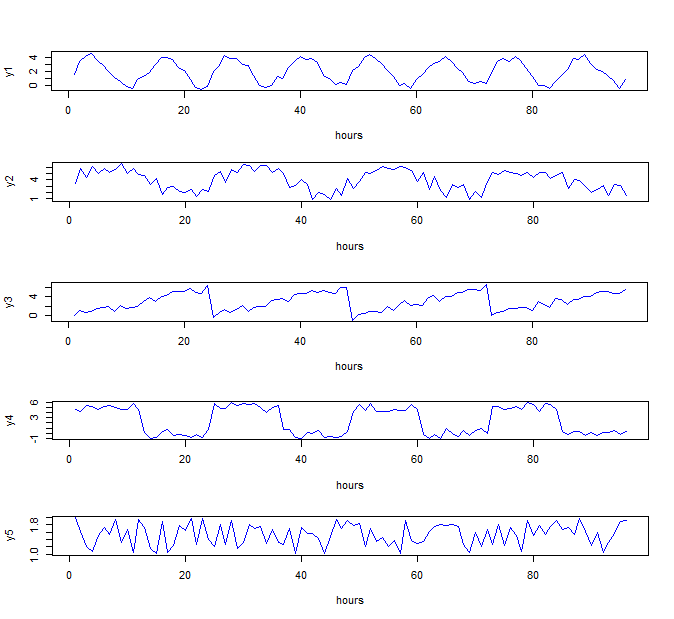
\includegraphics[scale=0.7]{Figures/synthetic data}
	\decoRule
	\caption[Synthetic Dataset]{Synthetic Dataset \parencite{own}}
	\label{fig:synthetic data}
\end{figure}

In a second step the dataset was enriched with six different kinds of anomalies. The anomalies embedded into the dataset are of type deviant cycle, temporary change and level shift. Figure \ref{fig:anomalies} shows examples of the embedded anomalies. The same kind of anomalies were embedded into the training and the test dataset.

\begin{figure}[h]
	\centering
	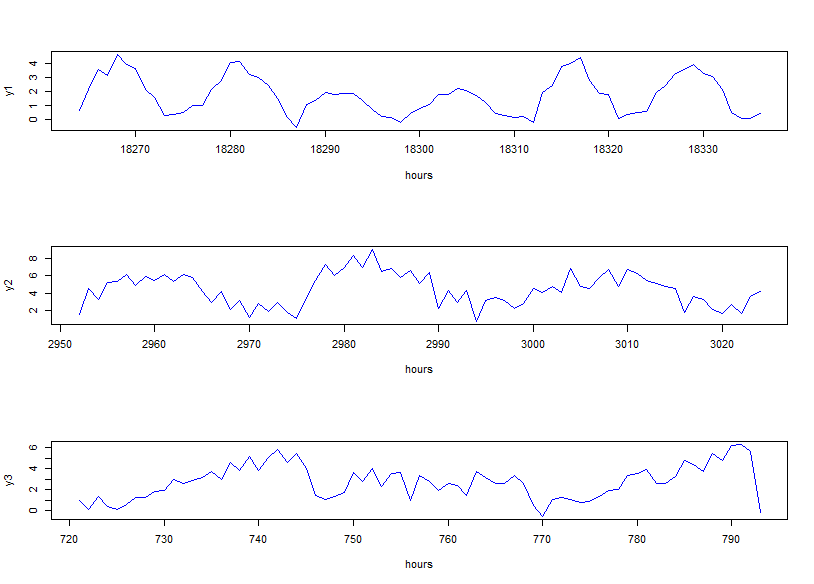
\includegraphics[scale=0.7]{Figures/Anomalies}
	\decoRule
	\caption[Synthetic Anomalies]{Synthetic Anomalies \parencite{own}}
	\label{fig:anomalies}
\end{figure}

For the supervised learning approach the dataset was also labelled. In each case the whole day was marked as an anomaly. In total 30 anomalous days were embedded into the dataset, this corresponds to 1.5 percent of anomalous datapoints.

\subsubsection{Neural Networks}
In the first experiment, a CNN was tested against a RNN in a supervised and also in an unsupervised fashion. As RNN, the type GRU was chosen. As some first attempts showed, that it showed sufficient results with improved computation time compared to the more complex LSTM. 

For the supervised learning approach, the chosen architecture can be seen in table \ref{Tab:Supervised Learning1}. 

\begin{table}[h]
\caption{Supervised Learning}
	\begin{center}
		\begin{tabular}{ | c | c | c | c |}
			\hline
			\thead{} & \thead{Input} & \thead{NN-Architecture} & \thead{Output} \\
			\hline
			\thead{CNN} &  120 past datapoints  & \makecell{2 1D-Convolutional Layers \\ 2 Max-Pooling Layers \\ 1 Dense Layer}  & \makecell{1 Dense Layer \\ with Sigmoid Activation}   \\
			\hline
			\thead{RNN} &  120 past datapoints  & \makecell{2 GRU Layers \\ 1 Dense Layer}  & \makecell{1 Dense Layer \\ with Sigmoid Activation}  \\
			\hline
		\end{tabular}
		\label{Tab:Supervised Learning1}
	\end{center}
\end{table}

 
The architecture used for the unsupervised learning approach, displayed in table \ref{Tab:Unupervised Learning1}, looked very similar. The main difference between the two architectures was that the CNN was not built as a sequential model. Instead of having one output layer, the CNN has five parallel output layers, each predicting a time series \footnote{More detailed summaries of the models can be found in appendix \ref{AppendixA}}.     

\begin{table}[h]
	\caption{Unupervised Learning}
	\begin{center}
		\begin{tabular}{ | c | c | c | c |}
			\hline
			\thead{} & \thead{Input} & \thead{NN-Architecture} & \thead{Output} \\
			\hline
			\thead{CNN} &  120 past datapoints  & \makecell{2 1D-Convolutional Layers \\ 2 Max-Pooling Layers }  & \makecell{ 5 Dense Layers with \\ 1 regression outputs}   \\
			\hline
			\thead{RNN} &  120 past datapoints  & \makecell{2 GRU Layers}  & \makecell{ 1 Dense Layers with \\ 5 regression outputs}  \\
			\hline
		\end{tabular}
	\label{Tab:Unupervised Learning1}
	\end{center}
\end{table}

\subsubsection{Results}

Inference time and F1-Score are, for all models, calculated on the same test dataset. As the initial dataset, it consists of 48000 datapoints, with 30 anomalous days embedded. For the supervised approach using a RNN, no F1-Score is reported, as the model, just like the trivial null classifier, always predicted no anomaly. Since the anomalies span over a whole day, for all approaches, the results were averaged per day. Resulting in normal or anomalous days. The reported F1-Score was finally calculated on this data. 


\begin{table}[h]
	\caption{Results}
	\begin{center}
		\begin{tabular}{ | c | c | c | c |}
			\hline
			\thead{} & \thead{F1-Score} & \thead{Training Time} & \thead{Inference Time} \\
			\hline
			\thead{CNN Supervised} &  0.991388  & 169s  & 422s   \\
			\hline
			\thead{RNN Supervised} &  -  & 967s   & 952s   \\
			\hline
			\thead{CNN Unsupervised} & 0.9989817  & 129s   & 435s   \\
			\hline
			\thead{RNN Unsupervised} &  0.9979613  & 300s   & 793s   \\
			\hline
			\thead{Trivial Null Classifier} &  0.9924204  & -  & -  \\
			\hline
		\end{tabular}
		\label{Tab:Results1}
	\end{center}
\end{table}

From the table \ref{Tab:Results1}, it can be seen that the supervised learning approach takes longer to train. This can be explained by the fact that a CNN must first learn the patterns and only then begins to recognise the anomalies. Further, it shows that despite promising results when training, the trivial null classifier achieves a higher F1-Score than the supervised CNN approach. 
The best score was achieved with a CNN applied in an unsupervised fashion. The CNN reported just one false negative and a false positive, compared to one false negative and two false positives of the RNN.

\newpage

\subsection{Experiment 2}
In a second experiment, a real dataset was used as base. The anomalies were embedded manually. Since, the unsupervised approach with RNN in Experiment 1 proved useless it was not included in the second experiment. Since the anomalies in training and test set were the same in Experiment 1, the CNN supervised was able to recognize some of the anomalies. In the second approach, it should be checked if this is approach could be of any use, if the anomalies consist of a hitherto unknown pattern.

\subsubsection{Dataset}
The dataset used was derived from the "Appliances Energy Prediction Dataset" available on the UCI Machine Learning Repository. The dataset consists of 9 room temperatures and corresponding humidity levels, energy in use of ligth and appliances, two random variables as well as six variables containing weather information. The dataset consists of 19735 datapoints, where 6 datapoints are drawn per hour. Of the available variables only 10 variables were used for the anomaly detection task. The variables used are 5 room temperatures, energy use, outside temperature, air pressure and wind speed. The variables were selected because they show a dependency. For example, a high outside temperature and energy use result in high temperatures in the different rooms. Figure \ref{fig:temp_dataset} provides an insight on the used dataset. 

\begin{figure}[h]
	\centering
	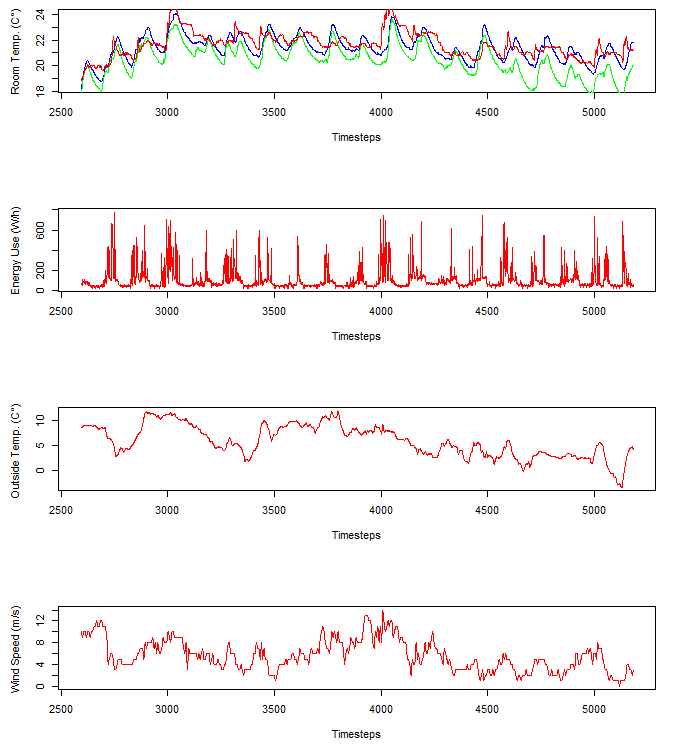
\includegraphics[scale=0.6]{Figures/temp_dataset}
	\decoRule
	\caption[Temperature Dataset]{Appliances Energy Prediction Dataset \parencite{Own or UCI???}}
	\label{fig:temp_dataset}
\end{figure}

Again, the anomalies were embedded manually into the dataset. The anomalies are of type level shift, deviant cycles, variaton change and distribution-based aggregate anomaly. The anomalies were embedded into the room temperature variables and the energy use variable. Figure \ref{fig:temp_anomalies} shows examples of the mentioned anomalies.

\begin{figure}[h]
	\centering
	\includegraphics[scale=0.7]{Figures/temp_anomalies}
	\decoRule
	\caption[Temperature Dataset Anomalies]{Examples of Embedded Anomalies \parencite{Own}}
	\label{fig:temp_anomalies}
\end{figure}




\subsection{Experiment 3}
